\documentclass[1p]{elsarticle_modified}
%\bibliographystyle{elsarticle-num}

%\usepackage[colorlinks]{hyperref}
%\usepackage{abbrmath_seonhwa} %\Abb, \Ascr, \Acal ,\Abf, \Afrak
\usepackage{amsfonts}
\usepackage{amssymb}
\usepackage{amsmath}
\usepackage{amsthm}
\usepackage{scalefnt}
\usepackage{amsbsy}
\usepackage{kotex}
\usepackage{caption}
\usepackage{subfig}
\usepackage{color}
\usepackage{graphicx}
\usepackage{xcolor} %% white, black, red, green, blue, cyan, magenta, yellow
\usepackage{float}
\usepackage{setspace}
\usepackage{hyperref}

\usepackage{tikz}
\usetikzlibrary{arrows}

\usepackage{multirow}
\usepackage{array} % fixed length table
\usepackage{hhline}

%%%%%%%%%%%%%%%%%%%%%
\makeatletter
\renewcommand*\env@matrix[1][\arraystretch]{%
	\edef\arraystretch{#1}%
	\hskip -\arraycolsep
	\let\@ifnextchar\new@ifnextchar
	\array{*\c@MaxMatrixCols c}}
\makeatother %https://tex.stackexchange.com/questions/14071/how-can-i-increase-the-line-spacing-in-a-matrix
%%%%%%%%%%%%%%%

\usepackage[normalem]{ulem}

\newcommand{\msout}[1]{\ifmmode\text{\sout{\ensuremath{#1}}}\else\sout{#1}\fi}
%SOURCE: \msout is \stkout macro in https://tex.stackexchange.com/questions/20609/strikeout-in-math-mode

\newcommand{\cancel}[1]{
	\ifmmode
	{\color{red}\msout{#1}}
	\else
	{\color{red}\sout{#1}}
	\fi
}

\newcommand{\add}[1]{
	{\color{blue}\uwave{#1}}
}

\newcommand{\replace}[2]{
	\ifmmode
	{\color{red}\msout{#1}}{\color{blue}\uwave{#2}}
	\else
	{\color{red}\sout{#1}}{\color{blue}\uwave{#2}}
	\fi
}

\newcommand{\Sol}{\mathcal{S}} %segment
\newcommand{\D}{D} %diagram
\newcommand{\A}{\mathcal{A}} %arc


%%%%%%%%%%%%%%%%%%%%%%%%%%%%%5 test

\def\sl{\operatorname{\textup{SL}}(2,\Cbb)}
\def\psl{\operatorname{\textup{PSL}}(2,\Cbb)}
\def\quan{\mkern 1mu \triangleright \mkern 1mu}

\theoremstyle{definition}
\newtheorem{thm}{Theorem}[section]
\newtheorem{prop}[thm]{Proposition}
\newtheorem{lem}[thm]{Lemma}
\newtheorem{ques}[thm]{Question}
\newtheorem{cor}[thm]{Corollary}
\newtheorem{defn}[thm]{Definition}
\newtheorem{exam}[thm]{Example}
\newtheorem{rmk}[thm]{Remark}
\newtheorem{alg}[thm]{Algorithm}

\newcommand{\I}{\sqrt{-1}}
\begin{document}

%\begin{frontmatter}
%
%\title{Boundary parabolic representations of knots up to 8 crossings}
%
%%% Group authors per affiliation:
%\author{Yunhi Cho} 
%\address{Department of Mathematics, University of Seoul, Seoul, Korea}
%\ead{yhcho@uos.ac.kr}
%
%
%\author{Seonhwa Kim} %\fnref{s_kim}}
%\address{Center for Geometry and Physics, Institute for Basic Science, Pohang, 37673, Korea}
%\ead{ryeona17@ibs.re.kr}
%
%\author{Hyuk Kim}
%\address{Department of Mathematical Sciences, Seoul National University, Seoul 08826, Korea}
%\ead{hyukkim@snu.ac.kr}
%
%\author{Seokbeom Yoon}
%\address{Department of Mathematical Sciences, Seoul National University, Seoul, 08826,  Korea}
%\ead{sbyoon15@snu.ac.kr}
%
%\begin{abstract}
%We find all boundary parabolic representation of knots up to 8 crossings.
%
%\end{abstract}
%\begin{keyword}
%    \MSC[2010] 57M25 
%\end{keyword}
%
%\end{frontmatter}

%\linenumbers
%\tableofcontents
%
\newcommand\colored[1]{\textcolor{white}{\rule[-0.35ex]{0.8em}{1.4ex}}\kern-0.8em\color{red} #1}%
%\newcommand\colored[1]{\textcolor{white}{ #1}\kern-2.17ex	\textcolor{white}{ #1}\kern-1.81ex	\textcolor{white}{ #1}\kern-2.15ex\color{red}#1	}

{\Large $\underline{12a_{0017}~(K12a_{0017})}$}

\setlength{\tabcolsep}{10pt}
\renewcommand{\arraystretch}{1.6}
\vspace{1cm}\begin{tabular}{m{100pt}>{\centering\arraybackslash}m{274pt}}
\multirow{5}{120pt}{
	\centering
	\includegraphics[width=112pt]{../../../GIT/diagram.site/Diagrams/png/818_12a_0017.png}\\
\ \ \ A knot diagram\footnotemark}&
\allowdisplaybreaks
\textbf{Linearized knot diagam} \\
\cline{2-2}
 &
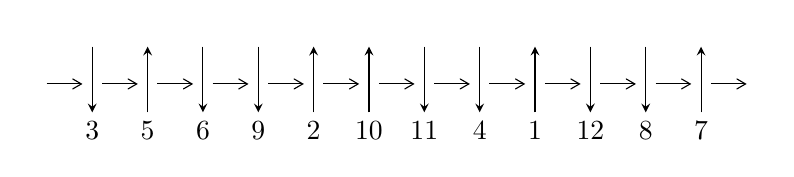
\begin{tikzpicture}[x=20pt, y=17pt]
	% nodes
	\node (C0) at (0, 0) {};
	\node (C1) at (1, 0) {};
	\node (C1U) at (1, +1) {};
	\node (C1D) at (1, -1) {3};

	\node (C2) at (2, 0) {};
	\node (C2U) at (2, +1) {};
	\node (C2D) at (2, -1) {5};

	\node (C3) at (3, 0) {};
	\node (C3U) at (3, +1) {};
	\node (C3D) at (3, -1) {6};

	\node (C4) at (4, 0) {};
	\node (C4U) at (4, +1) {};
	\node (C4D) at (4, -1) {9};

	\node (C5) at (5, 0) {};
	\node (C5U) at (5, +1) {};
	\node (C5D) at (5, -1) {2};

	\node (C6) at (6, 0) {};
	\node (C6U) at (6, +1) {};
	\node (C6D) at (6, -1) {10};

	\node (C7) at (7, 0) {};
	\node (C7U) at (7, +1) {};
	\node (C7D) at (7, -1) {11};

	\node (C8) at (8, 0) {};
	\node (C8U) at (8, +1) {};
	\node (C8D) at (8, -1) {4};

	\node (C9) at (9, 0) {};
	\node (C9U) at (9, +1) {};
	\node (C9D) at (9, -1) {1};

	\node (C10) at (10, 0) {};
	\node (C10U) at (10, +1) {};
	\node (C10D) at (10, -1) {12};

	\node (C11) at (11, 0) {};
	\node (C11U) at (11, +1) {};
	\node (C11D) at (11, -1) {8};

	\node (C12) at (12, 0) {};
	\node (C12U) at (12, +1) {};
	\node (C12D) at (12, -1) {7};
	\node (C13) at (13, 0) {};

	% arrows
	\draw[->,>={angle 60}]
	(C0) edge (C1) (C1) edge (C2) (C2) edge (C3) (C3) edge (C4) (C4) edge (C5) (C5) edge (C6) (C6) edge (C7) (C7) edge (C8) (C8) edge (C9) (C9) edge (C10) (C10) edge (C11) (C11) edge (C12) (C12) edge (C13) ;	\draw[->,>=stealth]
	(C1U) edge (C1D) (C2D) edge (C2U) (C3U) edge (C3D) (C4U) edge (C4D) (C5D) edge (C5U) (C6D) edge (C6U) (C7U) edge (C7D) (C8U) edge (C8D) (C9D) edge (C9U) (C10U) edge (C10D) (C11U) edge (C11D) (C12D) edge (C12U) ;
	\end{tikzpicture} \\
\hhline{~~} \\& 
\textbf{Solving Sequence} \\ \cline{2-2} 
 &
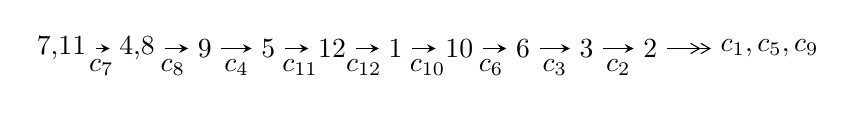
\begin{tikzpicture}[x=23pt, y=7pt]
	% node
	\node (A0) at (-1/8, 0) {7,11};
	\node (A1) at (17/16, 0) {4,8};
	\node (A2) at (17/8, 0) {9};
	\node (A3) at (25/8, 0) {5};
	\node (A4) at (33/8, 0) {12};
	\node (A5) at (41/8, 0) {1};
	\node (A6) at (49/8, 0) {10};
	\node (A7) at (57/8, 0) {6};
	\node (A8) at (65/8, 0) {3};
	\node (A9) at (73/8, 0) {2};
	\node (C1) at (1/2, -1) {$c_{7}$};
	\node (C2) at (13/8, -1) {$c_{8}$};
	\node (C3) at (21/8, -1) {$c_{4}$};
	\node (C4) at (29/8, -1) {$c_{11}$};
	\node (C5) at (37/8, -1) {$c_{12}$};
	\node (C6) at (45/8, -1) {$c_{10}$};
	\node (C7) at (53/8, -1) {$c_{6}$};
	\node (C8) at (61/8, -1) {$c_{3}$};
	\node (C9) at (69/8, -1) {$c_{2}$};
	\node (A10) at (11, 0) {$c_{1},c_{5},c_{9}$};

	% edge
	\draw[->,>=stealth]	
	(A0) edge (A1) (A1) edge (A2) (A2) edge (A3) (A3) edge (A4) (A4) edge (A5) (A5) edge (A6) (A6) edge (A7) (A7) edge (A8) (A8) edge (A9) ;
	\draw[->>,>={angle 60}]	
	(A9) edge (A10);
\end{tikzpicture} \\ 

\end{tabular} \\

\footnotetext{
The image of knot diagram is generated by the software ``\textbf{Draw programme}" developed by Andrew Bartholomew(\url{http://www.layer8.co.uk/maths/draw/index.htm\#Running-draw}), where we modified some parts for our purpose(\url{https://github.com/CATsTAILs/LinksPainter}).
}\phantom \\ \newline 
\centering \textbf{Ideals for irreducible components\footnotemark of $X_{\text{par}}$} 
 
\begin{align*}
I^u_{1}&=\langle 
u^{122}+5 u^{121}+\cdots+2 b-8,\;-17 u^{122}+41 u^{121}+\cdots+2 a-15,\;u^{123}-3 u^{122}+\cdots+2 u-1\rangle \\
I^u_{2}&=\langle 
- u^2 a+b,\;- u^4 a- u^3 a+u^2 a- u^3+a^2+a u- u^2+1,\;u^6+u^5- u^4-2 u^3+u+1\rangle \\
\\
\end{align*}
\raggedright * 2 irreducible components of $\dim_{\mathbb{C}}=0$, with total 135 representations.\\
\footnotetext{All coefficients of polynomials are rational numbers. But the coefficients are sometimes approximated in decimal forms when there is not enough margin.}
\newpage
\renewcommand{\arraystretch}{1}
\centering \section*{I. $I^u_{1}= \langle u^{122}+5 u^{121}+\cdots+2 b-8,\;-17 u^{122}+41 u^{121}+\cdots+2 a-15,\;u^{123}-3 u^{122}+\cdots+2 u-1 \rangle$}
\flushleft \textbf{(i) Arc colorings}\\
\begin{tabular}{m{7pt} m{180pt} m{7pt} m{180pt} }
\flushright $a_{7}=$&$\begin{pmatrix}1\\0\end{pmatrix}$ \\
\flushright $a_{11}=$&$\begin{pmatrix}0\\u\end{pmatrix}$ \\
\flushright $a_{4}=$&$\begin{pmatrix}\frac{17}{2} u^{122}-\frac{41}{2} u^{121}+\cdots-11 u+\frac{15}{2}\\-\frac{1}{2} u^{122}-\frac{5}{2} u^{121}+\cdots+\frac{1}{2} u+4\end{pmatrix}$ \\
\flushright $a_{8}=$&$\begin{pmatrix}1\\u^2\end{pmatrix}$ \\
\flushright $a_{9}=$&$\begin{pmatrix}- u^{11}+2 u^9-2 u^7+u^3\\- u^{11}+3 u^9-4 u^7+3 u^5- u^3+u\end{pmatrix}$ \\
\flushright $a_{5}=$&$\begin{pmatrix}\frac{7}{2} u^{122}-\frac{11}{2} u^{121}+\cdots-3 u+\frac{1}{2}\\\frac{1}{2} u^{122}+\frac{1}{2} u^{121}+\cdots-\frac{5}{2} u^2+\frac{3}{2} u\end{pmatrix}$ \\
\flushright $a_{12}=$&$\begin{pmatrix}- u\\- u^3+u\end{pmatrix}$ \\
\flushright $a_{1}=$&$\begin{pmatrix}- u^3\\- u^3+u\end{pmatrix}$ \\
\flushright $a_{10}=$&$\begin{pmatrix}u^3\\u^5- u^3+u\end{pmatrix}$ \\
\flushright $a_{6}=$&$\begin{pmatrix}u^8- u^6+u^4+1\\u^{10}-2 u^8+3 u^6-2 u^4+u^2\end{pmatrix}$ \\
\flushright $a_{3}=$&$\begin{pmatrix}5 u^{122}-12 u^{121}+\cdots-5 u+\frac{9}{2}\\- u^{122}+29 u^{120}+\cdots+\frac{3}{2} u+2\end{pmatrix}$ \\
\flushright $a_{2}=$&$\begin{pmatrix}- u^{122}+2 u^{121}+\cdots+3 u-\frac{3}{2}\\\frac{1}{2} u^{119}-\frac{1}{2} u^{118}+\cdots-2 u^2+\frac{3}{2} u\end{pmatrix}$\\&\end{tabular}
\flushleft \textbf{(ii) Obstruction class $= -1$}\\~\\
\flushleft \textbf{(iii) Cusp Shapes $= -13 u^{122}+\frac{57}{2} u^{121}+\cdots+\frac{45}{2} u-14$}\\~\\
\newpage\renewcommand{\arraystretch}{1}
\flushleft \textbf{(iv) u-Polynomials at the component}\newline \\
\begin{tabular}{m{50pt}|m{274pt}}
Crossings & \hspace{64pt}u-Polynomials at each crossing \\
\hline $$\begin{aligned}c_{1}\end{aligned}$$&$\begin{aligned}
&u^{123}+61 u^{122}+\cdots-6 u-1
\end{aligned}$\\
\hline $$\begin{aligned}c_{2},c_{5}\end{aligned}$$&$\begin{aligned}
&u^{123}+7 u^{122}+\cdots+8 u+1
\end{aligned}$\\
\hline $$\begin{aligned}c_{3}\end{aligned}$$&$\begin{aligned}
&u^{123}-7 u^{122}+\cdots-128330 u+93361
\end{aligned}$\\
\hline $$\begin{aligned}c_{4},c_{8}\end{aligned}$$&$\begin{aligned}
&u^{123}- u^{122}+\cdots+4096 u+4096
\end{aligned}$\\
\hline $$\begin{aligned}c_{6}\end{aligned}$$&$\begin{aligned}
&u^{123}-3 u^{122}+\cdots-10870 u+2425
\end{aligned}$\\
\hline $$\begin{aligned}c_{7},c_{11}\end{aligned}$$&$\begin{aligned}
&u^{123}+3 u^{122}+\cdots+2 u+1
\end{aligned}$\\
\hline $$\begin{aligned}c_{9}\end{aligned}$$&$\begin{aligned}
&u^{123}+13 u^{122}+\cdots+429074 u+27289
\end{aligned}$\\
\hline $$\begin{aligned}c_{10}\end{aligned}$$&$\begin{aligned}
&u^{123}+59 u^{122}+\cdots-2 u+1
\end{aligned}$\\
\hline $$\begin{aligned}c_{12}\end{aligned}$$&$\begin{aligned}
&u^{123}+9 u^{122}+\cdots+4066 u+1237
\end{aligned}$\\
\hline
\end{tabular}\\~\\
\newpage\renewcommand{\arraystretch}{1}
\flushleft \textbf{(v) Riley Polynomials at the component}\newline \\
\begin{tabular}{m{50pt}|m{274pt}}
Crossings & \hspace{64pt}Riley Polynomials at each crossing \\
\hline $$\begin{aligned}c_{1}\end{aligned}$$&$\begin{aligned}
&y^{123}+9 y^{122}+\cdots-14 y-1
\end{aligned}$\\
\hline $$\begin{aligned}c_{2},c_{5}\end{aligned}$$&$\begin{aligned}
&y^{123}+61 y^{122}+\cdots-6 y-1
\end{aligned}$\\
\hline $$\begin{aligned}c_{3}\end{aligned}$$&$\begin{aligned}
&y^{123}-43 y^{122}+\cdots-33652263950 y-8716276321
\end{aligned}$\\
\hline $$\begin{aligned}c_{4},c_{8}\end{aligned}$$&$\begin{aligned}
&y^{123}-65 y^{122}+\cdots+419430400 y-16777216
\end{aligned}$\\
\hline $$\begin{aligned}c_{6}\end{aligned}$$&$\begin{aligned}
&y^{123}-19 y^{122}+\cdots+113874350 y-5880625
\end{aligned}$\\
\hline $$\begin{aligned}c_{7},c_{11}\end{aligned}$$&$\begin{aligned}
&y^{123}-59 y^{122}+\cdots-2 y-1
\end{aligned}$\\
\hline $$\begin{aligned}c_{9}\end{aligned}$$&$\begin{aligned}
&y^{123}+41 y^{122}+\cdots-732678681206 y-744689521
\end{aligned}$\\
\hline $$\begin{aligned}c_{10}\end{aligned}$$&$\begin{aligned}
&y^{123}+13 y^{122}+\cdots-14 y-1
\end{aligned}$\\
\hline $$\begin{aligned}c_{12}\end{aligned}$$&$\begin{aligned}
&y^{123}+33 y^{122}+\cdots-130598898 y-1530169
\end{aligned}$\\
\hline
\end{tabular}\\~\\
\newpage\flushleft \textbf{(vi) Complex Volumes and Cusp Shapes}
$$\begin{array}{c|c|c}  
\text{Solutions to }I^u_{1}& \I (\text{vol} + \sqrt{-1}CS) & \text{Cusp shape}\\
 \hline 
\begin{aligned}
u &= \phantom{-}0.854485 + 0.561421 I \\
a &= \phantom{-}0.003316 - 0.563932 I \\
b &= -0.626981 + 0.060520 I\end{aligned}
 & -4.46926 - 2.02015 I & \phantom{-0.000000 } 0 \\ \hline\begin{aligned}
u &= \phantom{-}0.854485 - 0.561421 I \\
a &= \phantom{-}0.003316 + 0.563932 I \\
b &= -0.626981 - 0.060520 I\end{aligned}
 & -4.46926 + 2.02015 I & \phantom{-0.000000 } 0 \\ \hline\begin{aligned}
u &= \phantom{-}1.033990 + 0.061446 I \\
a &= \phantom{-}1.025610 + 0.127051 I \\
b &= \phantom{-}0.0245682 + 0.0714771 I\end{aligned}
 & -4.13307 - 3.64032 I & \phantom{-0.000000 } 0 \\ \hline\begin{aligned}
u &= \phantom{-}1.033990 - 0.061446 I \\
a &= \phantom{-}1.025610 - 0.127051 I \\
b &= \phantom{-}0.0245682 - 0.0714771 I\end{aligned}
 & -4.13307 + 3.64032 I & \phantom{-0.000000 } 0 \\ \hline\begin{aligned}
u &= \phantom{-}1.019840 + 0.221186 I \\
a &= -0.572632 - 0.294367 I \\
b &= \phantom{-}0.092325 - 0.139506 I\end{aligned}
 & -1.90019 - 0.28526 I & \phantom{-0.000000 } 0 \\ \hline\begin{aligned}
u &= \phantom{-}1.019840 - 0.221186 I \\
a &= -0.572632 + 0.294367 I \\
b &= \phantom{-}0.092325 + 0.139506 I\end{aligned}
 & -1.90019 + 0.28526 I & \phantom{-0.000000 } 0 \\ \hline\begin{aligned}
u &= \phantom{-}0.657781 + 0.664492 I \\
a &= -0.27330 + 1.72372 I \\
b &= -0.297545 + 0.371755 I\end{aligned}
 & -1.85277 - 10.74350 I & \phantom{-0.000000 } 0 \\ \hline\begin{aligned}
u &= \phantom{-}0.657781 - 0.664492 I \\
a &= -0.27330 - 1.72372 I \\
b &= -0.297545 - 0.371755 I\end{aligned}
 & -1.85277 + 10.74350 I & \phantom{-0.000000 } 0 \\ \hline\begin{aligned}
u &= \phantom{-}0.687369 + 0.623539 I \\
a &= -0.29318 + 1.44183 I \\
b &= -0.048159 + 0.259545 I\end{aligned}
 & -3.96911 - 2.64638 I & \phantom{-0.000000 } 0 \\ \hline\begin{aligned}
u &= \phantom{-}0.687369 - 0.623539 I \\
a &= -0.29318 - 1.44183 I \\
b &= -0.048159 - 0.259545 I\end{aligned}
 & -3.96911 + 2.64638 I & \phantom{-0.000000 } 0\\
 \hline 
 \end{array}$$\newpage$$\begin{array}{c|c|c}  
\text{Solutions to }I^u_{1}& \I (\text{vol} + \sqrt{-1}CS) & \text{Cusp shape}\\
 \hline 
\begin{aligned}
u &= \phantom{-}0.917903 + 0.565000 I \\
a &= \phantom{-}0.082196 + 0.192568 I \\
b &= \phantom{-}0.905526 - 0.344687 I\end{aligned}
 & -0.166656 + 0.924245 I & \phantom{-0.000000 } 0 \\ \hline\begin{aligned}
u &= \phantom{-}0.917903 - 0.565000 I \\
a &= \phantom{-}0.082196 - 0.192568 I \\
b &= \phantom{-}0.905526 + 0.344687 I\end{aligned}
 & -0.166656 - 0.924245 I & \phantom{-0.000000 } 0 \\ \hline\begin{aligned}
u &= -0.962014 + 0.501805 I \\
a &= \phantom{-}1.14651 + 1.46118 I \\
b &= \phantom{-}1.71891 + 0.68501 I\end{aligned}
 & -0.279306 - 0.572542 I & \phantom{-0.000000 } 0 \\ \hline\begin{aligned}
u &= -0.962014 - 0.501805 I \\
a &= \phantom{-}1.14651 - 1.46118 I \\
b &= \phantom{-}1.71891 - 0.68501 I\end{aligned}
 & -0.279306 + 0.572542 I & \phantom{-0.000000 } 0 \\ \hline\begin{aligned}
u &= \phantom{-}0.648152 + 0.645593 I \\
a &= \phantom{-}0.38530 - 1.67689 I \\
b &= \phantom{-}0.281699 - 0.248240 I\end{aligned}
 & \phantom{-}0.62783 - 5.66862 I & \phantom{-0.000000 } 0 \\ \hline\begin{aligned}
u &= \phantom{-}0.648152 - 0.645593 I \\
a &= \phantom{-}0.38530 + 1.67689 I \\
b &= \phantom{-}0.281699 + 0.248240 I\end{aligned}
 & \phantom{-}0.62783 + 5.66862 I & \phantom{-0.000000 } 0 \\ \hline\begin{aligned}
u &= \phantom{-}0.912418 + 0.590250 I \\
a &= -0.263358 - 0.252976 I \\
b &= -1.030770 + 0.176984 I\end{aligned}
 & -2.60544 + 5.87088 I & \phantom{-0.000000 } 0 \\ \hline\begin{aligned}
u &= \phantom{-}0.912418 - 0.590250 I \\
a &= -0.263358 + 0.252976 I \\
b &= -1.030770 - 0.176984 I\end{aligned}
 & -2.60544 - 5.87088 I & \phantom{-0.000000 } 0 \\ \hline\begin{aligned}
u &= \phantom{-}1.048540 + 0.385425 I \\
a &= \phantom{-}0.433108 - 0.660989 I \\
b &= \phantom{-}0.422710 + 0.320271 I\end{aligned}
 & -3.06638 - 1.39605 I & \phantom{-0.000000 } 0 \\ \hline\begin{aligned}
u &= \phantom{-}1.048540 - 0.385425 I \\
a &= \phantom{-}0.433108 + 0.660989 I \\
b &= \phantom{-}0.422710 - 0.320271 I\end{aligned}
 & -3.06638 + 1.39605 I & \phantom{-0.000000 } 0\\
 \hline 
 \end{array}$$\newpage$$\begin{array}{c|c|c}  
\text{Solutions to }I^u_{1}& \I (\text{vol} + \sqrt{-1}CS) & \text{Cusp shape}\\
 \hline 
\begin{aligned}
u &= \phantom{-}0.985605 + 0.527401 I \\
a &= -0.412366 - 0.202768 I \\
b &= \phantom{-}0.696926 - 1.116170 I\end{aligned}
 & \phantom{-}1.30652 - 1.06855 I & \phantom{-0.000000 } 0 \\ \hline\begin{aligned}
u &= \phantom{-}0.985605 - 0.527401 I \\
a &= -0.412366 + 0.202768 I \\
b &= \phantom{-}0.696926 + 1.116170 I\end{aligned}
 & \phantom{-}1.30652 + 1.06855 I & \phantom{-0.000000 } 0 \\ \hline\begin{aligned}
u &= \phantom{-}1.087640 + 0.274343 I \\
a &= -0.353683 - 0.740293 I \\
b &= \phantom{-}0.250172 - 0.184177 I\end{aligned}
 & -2.47005 - 0.30272 I & \phantom{-0.000000 } 0 \\ \hline\begin{aligned}
u &= \phantom{-}1.087640 - 0.274343 I \\
a &= -0.353683 + 0.740293 I \\
b &= \phantom{-}0.250172 + 0.184177 I\end{aligned}
 & -2.47005 + 0.30272 I & \phantom{-0.000000 } 0 \\ \hline\begin{aligned}
u &= -0.505350 + 0.716113 I \\
a &= \phantom{-}0.828458 + 0.277865 I \\
b &= \phantom{-}0.921356 - 0.358807 I\end{aligned}
 & \phantom{-}1.06865 - 4.56495 I & \phantom{-0.000000 } 0 \\ \hline\begin{aligned}
u &= -0.505350 - 0.716113 I \\
a &= \phantom{-}0.828458 - 0.277865 I \\
b &= \phantom{-}0.921356 + 0.358807 I\end{aligned}
 & \phantom{-}1.06865 + 4.56495 I & \phantom{-0.000000 } 0 \\ \hline\begin{aligned}
u &= -0.995492 + 0.532233 I \\
a &= -0.97900 - 1.25049 I \\
b &= -1.45523 - 0.58880 I\end{aligned}
 & \phantom{-}1.41929 + 3.95035 I & \phantom{-0.000000 } 0 \\ \hline\begin{aligned}
u &= -0.995492 - 0.532233 I \\
a &= -0.97900 + 1.25049 I \\
b &= -1.45523 + 0.58880 I\end{aligned}
 & \phantom{-}1.41929 - 3.95035 I & \phantom{-0.000000 } 0 \\ \hline\begin{aligned}
u &= -1.095060 + 0.295281 I \\
a &= \phantom{-}3.02439 + 0.12421 I \\
b &= \phantom{-}2.53218 - 1.86329 I\end{aligned}
 & -3.16948 + 2.81128 I & \phantom{-0.000000 } 0 \\ \hline\begin{aligned}
u &= -1.095060 - 0.295281 I \\
a &= \phantom{-}3.02439 - 0.12421 I \\
b &= \phantom{-}2.53218 + 1.86329 I\end{aligned}
 & -3.16948 - 2.81128 I & \phantom{-0.000000 } 0\\
 \hline 
 \end{array}$$\newpage$$\begin{array}{c|c|c}  
\text{Solutions to }I^u_{1}& \I (\text{vol} + \sqrt{-1}CS) & \text{Cusp shape}\\
 \hline 
\begin{aligned}
u &= -1.102410 + 0.267908 I \\
a &= -2.77281 + 0.10154 I \\
b &= -2.15753 + 2.01225 I\end{aligned}
 & -2.88698 - 2.46184 I & \phantom{-0.000000 } 0 \\ \hline\begin{aligned}
u &= -1.102410 - 0.267908 I \\
a &= -2.77281 - 0.10154 I \\
b &= -2.15753 - 2.01225 I\end{aligned}
 & -2.88698 + 2.46184 I & \phantom{-0.000000 } 0 \\ \hline\begin{aligned}
u &= -0.448019 + 0.736719 I \\
a &= \phantom{-}0.745796 - 0.073275 I \\
b &= \phantom{-}0.594549 - 0.660727 I\end{aligned}
 & \phantom{-}0.78043 + 2.03644 I & \phantom{-0.000000 } 0 \\ \hline\begin{aligned}
u &= -0.448019 - 0.736719 I \\
a &= \phantom{-}0.745796 + 0.073275 I \\
b &= \phantom{-}0.594549 + 0.660727 I\end{aligned}
 & \phantom{-}0.78043 - 2.03644 I & \phantom{-0.000000 } 0 \\ \hline\begin{aligned}
u &= \phantom{-}0.858281\phantom{ +0.000000I} \\
a &= -0.927426\phantom{ +0.000000I} \\
b &= \phantom{-}0.108938\phantom{ +0.000000I}\end{aligned}
 & -1.50207\phantom{ +0.000000I} & -5.95250\phantom{ +0.000000I} \\ \hline\begin{aligned}
u &= \phantom{-}1.017760 + 0.522481 I \\
a &= \phantom{-}0.811698 + 0.352586 I \\
b &= -0.44309 + 1.64463 I\end{aligned}
 & \phantom{-}0.27133 - 5.98593 I & \phantom{-0.000000 } 0 \\ \hline\begin{aligned}
u &= \phantom{-}1.017760 - 0.522481 I \\
a &= \phantom{-}0.811698 - 0.352586 I \\
b &= -0.44309 - 1.64463 I\end{aligned}
 & \phantom{-}0.27133 + 5.98593 I & \phantom{-0.000000 } 0 \\ \hline\begin{aligned}
u &= -0.621924 + 0.587387 I \\
a &= \phantom{-}0.727972 + 1.082340 I \\
b &= \phantom{-}1.223970 + 0.460141 I\end{aligned}
 & \phantom{-}0.70009 + 4.93753 I & \phantom{-0.000000 } 0 \\ \hline\begin{aligned}
u &= -0.621924 - 0.587387 I \\
a &= \phantom{-}0.727972 - 1.082340 I \\
b &= \phantom{-}1.223970 - 0.460141 I\end{aligned}
 & \phantom{-}0.70009 - 4.93753 I & \phantom{-0.000000 } 0 \\ \hline\begin{aligned}
u &= \phantom{-}0.326719 + 0.783768 I \\
a &= -0.60353 - 1.35303 I \\
b &= \phantom{-}2.26170 - 0.29466 I\end{aligned}
 & -3.54566 + 13.00910 I & \phantom{-0.000000 } 0. - 8.03983 I\\
 \hline 
 \end{array}$$\newpage$$\begin{array}{c|c|c}  
\text{Solutions to }I^u_{1}& \I (\text{vol} + \sqrt{-1}CS) & \text{Cusp shape}\\
 \hline 
\begin{aligned}
u &= \phantom{-}0.326719 - 0.783768 I \\
a &= -0.60353 + 1.35303 I \\
b &= \phantom{-}2.26170 + 0.29466 I\end{aligned}
 & -3.54566 - 13.00910 I & \phantom{-0.000000 -}0. + 8.03983 I \\ \hline\begin{aligned}
u &= \phantom{-}1.123590 + 0.265053 I \\
a &= \phantom{-}0.502221 + 0.942772 I \\
b &= -0.263992 + 0.306687 I\end{aligned}
 & -5.04425 + 3.82260 I & \phantom{-0.000000 } 0 \\ \hline\begin{aligned}
u &= \phantom{-}1.123590 - 0.265053 I \\
a &= \phantom{-}0.502221 - 0.942772 I \\
b &= -0.263992 - 0.306687 I\end{aligned}
 & -5.04425 - 3.82260 I & \phantom{-0.000000 } 0 \\ \hline\begin{aligned}
u &= -0.510966 + 0.671472 I \\
a &= -0.654545 - 0.468997 I \\
b &= -0.869605 + 0.071896 I\end{aligned}
 & \phantom{-}2.93696 - 0.44778 I & \phantom{-0.000000 } 0 \\ \hline\begin{aligned}
u &= -0.510966 - 0.671472 I \\
a &= -0.654545 + 0.468997 I \\
b &= -0.869605 - 0.071896 I\end{aligned}
 & \phantom{-}2.93696 + 0.44778 I & \phantom{-0.000000 } 0 \\ \hline\begin{aligned}
u &= \phantom{-}1.119360 + 0.310725 I \\
a &= \phantom{-}0.185438 + 1.038430 I \\
b &= -0.432873 + 0.226764 I\end{aligned}
 & -5.53092 - 3.70026 I & \phantom{-0.000000 } 0 \\ \hline\begin{aligned}
u &= \phantom{-}1.119360 - 0.310725 I \\
a &= \phantom{-}0.185438 - 1.038430 I \\
b &= -0.432873 - 0.226764 I\end{aligned}
 & -5.53092 + 3.70026 I & \phantom{-0.000000 } 0 \\ \hline\begin{aligned}
u &= \phantom{-}0.324855 + 0.771366 I \\
a &= \phantom{-}0.72033 + 1.32461 I \\
b &= -2.21918 + 0.30802 I\end{aligned}
 & -0.98344 + 7.78701 I & \phantom{-0.000000 } 0. - 4.67811 I \\ \hline\begin{aligned}
u &= \phantom{-}0.324855 - 0.771366 I \\
a &= \phantom{-}0.72033 - 1.32461 I \\
b &= -2.21918 - 0.30802 I\end{aligned}
 & -0.98344 - 7.78701 I & \phantom{-0.000000 -}0. + 4.67811 I \\ \hline\begin{aligned}
u &= \phantom{-}0.581489 + 0.598075 I \\
a &= \phantom{-}0.89914 - 1.66803 I \\
b &= \phantom{-}0.309435 + 0.200315 I\end{aligned}
 & \phantom{-}2.49653 - 3.41082 I & \phantom{-0.000000 -}0. + 7.23745 I\\
 \hline 
 \end{array}$$\newpage$$\begin{array}{c|c|c}  
\text{Solutions to }I^u_{1}& \I (\text{vol} + \sqrt{-1}CS) & \text{Cusp shape}\\
 \hline 
\begin{aligned}
u &= \phantom{-}0.581489 - 0.598075 I \\
a &= \phantom{-}0.89914 + 1.66803 I \\
b &= \phantom{-}0.309435 - 0.200315 I\end{aligned}
 & \phantom{-}2.49653 + 3.41082 I & \phantom{-0.000000 } 0. - 7.23745 I \\ \hline\begin{aligned}
u &= -1.142960 + 0.238255 I \\
a &= -2.32696 - 0.11666 I \\
b &= -1.74160 + 1.67456 I\end{aligned}
 & -5.56302 - 4.94470 I & \phantom{-0.000000 } 0 \\ \hline\begin{aligned}
u &= -1.142960 - 0.238255 I \\
a &= -2.32696 + 0.11666 I \\
b &= -1.74160 - 1.67456 I\end{aligned}
 & -5.56302 + 4.94470 I & \phantom{-0.000000 } 0 \\ \hline\begin{aligned}
u &= -1.063460 + 0.492512 I \\
a &= \phantom{-}1.46708 + 0.61955 I \\
b &= \phantom{-}1.53045 - 0.21359 I\end{aligned}
 & -2.35808 + 5.38729 I & \phantom{-0.000000 } 0 \\ \hline\begin{aligned}
u &= -1.063460 - 0.492512 I \\
a &= \phantom{-}1.46708 - 0.61955 I \\
b &= \phantom{-}1.53045 + 0.21359 I\end{aligned}
 & -2.35808 - 5.38729 I & \phantom{-0.000000 } 0 \\ \hline\begin{aligned}
u &= \phantom{-}0.300988 + 0.770638 I \\
a &= -0.690849 - 1.102760 I \\
b &= \phantom{-}2.17376 - 0.22546 I\end{aligned}
 & -5.84365 + 4.55880 I & -6.44547 - 2.49035 I \\ \hline\begin{aligned}
u &= \phantom{-}0.300988 - 0.770638 I \\
a &= -0.690849 + 1.102760 I \\
b &= \phantom{-}2.17376 + 0.22546 I\end{aligned}
 & -5.84365 - 4.55880 I & -6.44547 + 2.49035 I \\ \hline\begin{aligned}
u &= -0.563362 + 0.602679 I \\
a &= -0.615246 - 0.881766 I \\
b &= -1.040120 - 0.318191 I\end{aligned}
 & \phantom{-}2.69193 + 0.55935 I & \phantom{-}3.98610 + 0. I\phantom{ +0.000000I} \\ \hline\begin{aligned}
u &= -0.563362 - 0.602679 I \\
a &= -0.615246 + 0.881766 I \\
b &= -1.040120 + 0.318191 I\end{aligned}
 & \phantom{-}2.69193 - 0.55935 I & \phantom{-}3.98610 + 0. I\phantom{ +0.000000I} \\ \hline\begin{aligned}
u &= -1.152950 + 0.230458 I \\
a &= \phantom{-}2.24298 + 0.18923 I \\
b &= \phantom{-}1.66975 - 1.59343 I\end{aligned}
 & -8.21753 - 10.13550 I & \phantom{-0.000000 } 0\\
 \hline 
 \end{array}$$\newpage$$\begin{array}{c|c|c}  
\text{Solutions to }I^u_{1}& \I (\text{vol} + \sqrt{-1}CS) & \text{Cusp shape}\\
 \hline 
\begin{aligned}
u &= -1.152950 - 0.230458 I \\
a &= \phantom{-}2.24298 - 0.18923 I \\
b &= \phantom{-}1.66975 + 1.59343 I\end{aligned}
 & -8.21753 + 10.13550 I & \phantom{-0.000000 } 0 \\ \hline\begin{aligned}
u &= -0.405700 + 0.715550 I \\
a &= -0.547830 + 0.258526 I \\
b &= -0.233364 + 0.680720 I\end{aligned}
 & \phantom{-}2.43695 - 1.70720 I & \phantom{-}1.69325 + 0. I\phantom{ +0.000000I} \\ \hline\begin{aligned}
u &= -0.405700 - 0.715550 I \\
a &= -0.547830 - 0.258526 I \\
b &= -0.233364 - 0.680720 I\end{aligned}
 & \phantom{-}2.43695 + 1.70720 I & \phantom{-}1.69325 + 0. I\phantom{ +0.000000I} \\ \hline\begin{aligned}
u &= -1.030200 + 0.571691 I \\
a &= -0.516402 - 1.134700 I \\
b &= -0.985503 - 0.722266 I\end{aligned}
 & \phantom{-}1.40801 + 5.27406 I & \phantom{-0.000000 } 0 \\ \hline\begin{aligned}
u &= -1.030200 - 0.571691 I \\
a &= -0.516402 + 1.134700 I \\
b &= -0.985503 + 0.722266 I\end{aligned}
 & \phantom{-}1.40801 - 5.27406 I & \phantom{-0.000000 } 0 \\ \hline\begin{aligned}
u &= -1.153290 + 0.256833 I \\
a &= \phantom{-}2.45010 + 0.23769 I \\
b &= \phantom{-}1.88125 - 1.56566 I\end{aligned}
 & -10.34180 - 1.56416 I & \phantom{-0.000000 } 0 \\ \hline\begin{aligned}
u &= -1.153290 - 0.256833 I \\
a &= \phantom{-}2.45010 - 0.23769 I \\
b &= \phantom{-}1.88125 + 1.56566 I\end{aligned}
 & -10.34180 + 1.56416 I & \phantom{-0.000000 } 0 \\ \hline\begin{aligned}
u &= -1.141170 + 0.345577 I \\
a &= \phantom{-}2.74400 + 0.42807 I \\
b &= \phantom{-}2.32803 - 1.27018 I\end{aligned}
 & -6.77873 + 4.44845 I & \phantom{-0.000000 } 0 \\ \hline\begin{aligned}
u &= -1.141170 - 0.345577 I \\
a &= \phantom{-}2.74400 - 0.42807 I \\
b &= \phantom{-}2.32803 + 1.27018 I\end{aligned}
 & -6.77873 - 4.44845 I & \phantom{-0.000000 } 0 \\ \hline\begin{aligned}
u &= -1.039880 + 0.593668 I \\
a &= \phantom{-}0.269757 + 1.286620 I \\
b &= \phantom{-}0.839442 + 0.975017 I\end{aligned}
 & -0.50937 + 9.58006 I & \phantom{-0.000000 } 0\\
 \hline 
 \end{array}$$\newpage$$\begin{array}{c|c|c}  
\text{Solutions to }I^u_{1}& \I (\text{vol} + \sqrt{-1}CS) & \text{Cusp shape}\\
 \hline 
\begin{aligned}
u &= -1.039880 - 0.593668 I \\
a &= \phantom{-}0.269757 - 1.286620 I \\
b &= \phantom{-}0.839442 - 0.975017 I\end{aligned}
 & -0.50937 - 9.58006 I & \phantom{-0.000000 } 0 \\ \hline\begin{aligned}
u &= -0.314117 + 0.738169 I \\
a &= \phantom{-}0.575358 - 0.604862 I \\
b &= -0.157550 - 1.089370 I\end{aligned}
 & -0.72558 - 6.64128 I & -2.45271 + 5.62875 I \\ \hline\begin{aligned}
u &= -0.314117 - 0.738169 I \\
a &= \phantom{-}0.575358 + 0.604862 I \\
b &= -0.157550 + 1.089370 I\end{aligned}
 & -0.72558 + 6.64128 I & -2.45271 - 5.62875 I \\ \hline\begin{aligned}
u &= -1.154440 + 0.326977 I \\
a &= -2.73063 - 0.39678 I \\
b &= -2.24616 + 1.33762 I\end{aligned}
 & -11.15920 + 0.73897 I & \phantom{-0.000000 } 0 \\ \hline\begin{aligned}
u &= -1.154440 - 0.326977 I \\
a &= -2.73063 + 0.39678 I \\
b &= -2.24616 - 1.33762 I\end{aligned}
 & -11.15920 - 0.73897 I & \phantom{-0.000000 } 0 \\ \hline\begin{aligned}
u &= \phantom{-}0.329435 + 0.722217 I \\
a &= \phantom{-}1.26469 + 1.24360 I \\
b &= -2.06959 + 0.45452 I\end{aligned}
 & \phantom{-}1.34347 + 5.13610 I & -0.89905 - 6.52878 I \\ \hline\begin{aligned}
u &= \phantom{-}0.329435 - 0.722217 I \\
a &= \phantom{-}1.26469 - 1.24360 I \\
b &= -2.06959 - 0.45452 I\end{aligned}
 & \phantom{-}1.34347 - 5.13610 I & -0.89905 + 6.52878 I \\ \hline\begin{aligned}
u &= -1.153440 + 0.356078 I \\
a &= -2.72091 - 0.41587 I \\
b &= -2.27381 + 1.22883 I\end{aligned}
 & -9.68798 + 9.41535 I & \phantom{-0.000000 } 0 \\ \hline\begin{aligned}
u &= -1.153440 - 0.356078 I \\
a &= -2.72091 + 0.41587 I \\
b &= -2.27381 - 1.22883 I\end{aligned}
 & -9.68798 - 9.41535 I & \phantom{-0.000000 } 0 \\ \hline\begin{aligned}
u &= -0.337945 + 0.711241 I \\
a &= -0.514362 + 0.535580 I \\
b &= \phantom{-}0.117785 + 0.912749 I\end{aligned}
 & \phantom{-}1.68112 - 2.28331 I & \phantom{-}2.01200 + 1.73250 I\\
 \hline 
 \end{array}$$\newpage$$\begin{array}{c|c|c}  
\text{Solutions to }I^u_{1}& \I (\text{vol} + \sqrt{-1}CS) & \text{Cusp shape}\\
 \hline 
\begin{aligned}
u &= -0.337945 - 0.711241 I \\
a &= -0.514362 - 0.535580 I \\
b &= \phantom{-}0.117785 - 0.912749 I\end{aligned}
 & \phantom{-}1.68112 + 2.28331 I & \phantom{-}2.01200 - 1.73250 I \\ \hline\begin{aligned}
u &= \phantom{-}0.531699 + 0.571261 I \\
a &= -1.31269 + 1.58049 I \\
b &= -0.189489 - 0.498823 I\end{aligned}
 & \phantom{-}1.71359 + 1.58676 I & -0.51367 + 2.12597 I \\ \hline\begin{aligned}
u &= \phantom{-}0.531699 - 0.571261 I \\
a &= -1.31269 - 1.58049 I \\
b &= -0.189489 + 0.498823 I\end{aligned}
 & \phantom{-}1.71359 - 1.58676 I & -0.51367 - 2.12597 I \\ \hline\begin{aligned}
u &= -1.074920 + 0.589470 I \\
a &= -0.231426 + 1.076660 I \\
b &= \phantom{-}0.305449 + 1.020630 I\end{aligned}
 & -1.06964 + 3.01381 I & \phantom{-0.000000 } 0 \\ \hline\begin{aligned}
u &= -1.074920 - 0.589470 I \\
a &= -0.231426 - 1.076660 I \\
b &= \phantom{-}0.305449 - 1.020630 I\end{aligned}
 & -1.06964 - 3.01381 I & \phantom{-0.000000 } 0 \\ \hline\begin{aligned}
u &= -1.089820 + 0.571745 I \\
a &= \phantom{-}0.566381 - 0.717391 I \\
b &= \phantom{-}0.140524 - 0.866907 I\end{aligned}
 & \phantom{-}0.42992 + 6.63920 I & \phantom{-0.000000 } 0 \\ \hline\begin{aligned}
u &= -1.089820 - 0.571745 I \\
a &= \phantom{-}0.566381 + 0.717391 I \\
b &= \phantom{-}0.140524 + 0.866907 I\end{aligned}
 & \phantom{-}0.42992 - 6.63920 I & \phantom{-0.000000 } 0 \\ \hline\begin{aligned}
u &= \phantom{-}1.111230 + 0.545507 I \\
a &= \phantom{-}2.45891 - 1.62700 I \\
b &= \phantom{-}3.32507 + 1.26226 I\end{aligned}
 & -1.45622 - 4.63554 I & \phantom{-0.000000 } 0 \\ \hline\begin{aligned}
u &= \phantom{-}1.111230 - 0.545507 I \\
a &= \phantom{-}2.45891 + 1.62700 I \\
b &= \phantom{-}3.32507 - 1.26226 I\end{aligned}
 & -1.45622 + 4.63554 I & \phantom{-0.000000 } 0 \\ \hline\begin{aligned}
u &= \phantom{-}0.323938 + 0.689603 I \\
a &= -1.58714 - 0.95579 I \\
b &= \phantom{-}1.89255 - 0.55461 I\end{aligned}
 & \phantom{-}0.818092 - 0.124046 I & -3.14780 - 0.83223 I\\
 \hline 
 \end{array}$$\newpage$$\begin{array}{c|c|c}  
\text{Solutions to }I^u_{1}& \I (\text{vol} + \sqrt{-1}CS) & \text{Cusp shape}\\
 \hline 
\begin{aligned}
u &= \phantom{-}0.323938 - 0.689603 I \\
a &= -1.58714 + 0.95579 I \\
b &= \phantom{-}1.89255 + 0.55461 I\end{aligned}
 & \phantom{-}0.818092 + 0.124046 I & -3.14780 + 0.83223 I \\ \hline\begin{aligned}
u &= \phantom{-}1.132130 + 0.504504 I \\
a &= \phantom{-}1.68573 - 1.49625 I \\
b &= \phantom{-}2.18204 + 0.67494 I\end{aligned}
 & -5.70491 - 3.44197 I & \phantom{-0.000000 } 0 \\ \hline\begin{aligned}
u &= \phantom{-}1.132130 - 0.504504 I \\
a &= \phantom{-}1.68573 + 1.49625 I \\
b &= \phantom{-}2.18204 - 0.67494 I\end{aligned}
 & -5.70491 + 3.44197 I & \phantom{-0.000000 } 0 \\ \hline\begin{aligned}
u &= -1.119960 + 0.532893 I \\
a &= -1.45764 + 0.36603 I \\
b &= -1.02362 + 0.98782 I\end{aligned}
 & -4.02319 + 3.95622 I & \phantom{-0.000000 } 0 \\ \hline\begin{aligned}
u &= -1.119960 - 0.532893 I \\
a &= -1.45764 - 0.36603 I \\
b &= -1.02362 - 0.98782 I\end{aligned}
 & -4.02319 - 3.95622 I & \phantom{-0.000000 } 0 \\ \hline\begin{aligned}
u &= -1.111910 + 0.553776 I \\
a &= \phantom{-}1.142580 - 0.571408 I \\
b &= \phantom{-}0.680128 - 1.006950 I\end{aligned}
 & -0.57041 + 7.12600 I & \phantom{-0.000000 } 0 \\ \hline\begin{aligned}
u &= -1.111910 - 0.553776 I \\
a &= \phantom{-}1.142580 + 0.571408 I \\
b &= \phantom{-}0.680128 + 1.006950 I\end{aligned}
 & -0.57041 - 7.12600 I & \phantom{-0.000000 } 0 \\ \hline\begin{aligned}
u &= \phantom{-}0.203285 + 0.729617 I \\
a &= \phantom{-}0.726731 + 0.322337 I \\
b &= -1.81310 - 0.11441 I\end{aligned}
 & -7.16219 + 2.64076 I & -7.80104 - 2.59513 I \\ \hline\begin{aligned}
u &= \phantom{-}0.203285 - 0.729617 I \\
a &= \phantom{-}0.726731 - 0.322337 I \\
b &= -1.81310 + 0.11441 I\end{aligned}
 & -7.16219 - 2.64076 I & -7.80104 + 2.59513 I \\ \hline\begin{aligned}
u &= \phantom{-}1.142870 + 0.494166 I \\
a &= -1.51219 + 1.59682 I \\
b &= -2.05783 - 0.43237 I\end{aligned}
 & -8.75415 + 1.36519 I & \phantom{-0.000000 } 0\\
 \hline 
 \end{array}$$\newpage$$\begin{array}{c|c|c}  
\text{Solutions to }I^u_{1}& \I (\text{vol} + \sqrt{-1}CS) & \text{Cusp shape}\\
 \hline 
\begin{aligned}
u &= \phantom{-}1.142870 - 0.494166 I \\
a &= -1.51219 - 1.59682 I \\
b &= -2.05783 + 0.43237 I\end{aligned}
 & -8.75415 - 1.36519 I & \phantom{-0.000000 } 0 \\ \hline\begin{aligned}
u &= \phantom{-}1.116840 + 0.555196 I \\
a &= -2.40203 + 1.83735 I \\
b &= -3.52952 - 0.89285 I\end{aligned}
 & -0.94884 - 10.00770 I & \phantom{-0.000000 } 0 \\ \hline\begin{aligned}
u &= \phantom{-}1.116840 - 0.555196 I \\
a &= -2.40203 - 1.83735 I \\
b &= -3.52952 + 0.89285 I\end{aligned}
 & -0.94884 + 10.00770 I & \phantom{-0.000000 } 0 \\ \hline\begin{aligned}
u &= -1.124970 + 0.555762 I \\
a &= -1.31913 + 0.71542 I \\
b &= -0.75747 + 1.20075 I\end{aligned}
 & -3.08943 + 11.54780 I & \phantom{-0.000000 } 0 \\ \hline\begin{aligned}
u &= -1.124970 - 0.555762 I \\
a &= -1.31913 - 0.71542 I \\
b &= -0.75747 - 1.20075 I\end{aligned}
 & -3.08943 - 11.54780 I & \phantom{-0.000000 } 0 \\ \hline\begin{aligned}
u &= \phantom{-}1.143390 + 0.517843 I \\
a &= -1.79911 + 1.70410 I \\
b &= -2.47710 - 0.50435 I\end{aligned}
 & -9.86641 - 7.31652 I & \phantom{-0.000000 } 0 \\ \hline\begin{aligned}
u &= \phantom{-}1.143390 - 0.517843 I \\
a &= -1.79911 - 1.70410 I \\
b &= -2.47710 + 0.50435 I\end{aligned}
 & -9.86641 + 7.31652 I & \phantom{-0.000000 } 0 \\ \hline\begin{aligned}
u &= -0.271121 + 0.683887 I \\
a &= \phantom{-}0.479920 - 0.674630 I \\
b &= -0.416798 - 0.951510 I\end{aligned}
 & -1.60447 + 0.71899 I & -4.24680 - 0.96822 I \\ \hline\begin{aligned}
u &= -0.271121 - 0.683887 I \\
a &= \phantom{-}0.479920 + 0.674630 I \\
b &= -0.416798 + 0.951510 I\end{aligned}
 & -1.60447 - 0.71899 I & -4.24680 + 0.96822 I \\ \hline\begin{aligned}
u &= \phantom{-}1.131700 + 0.568256 I \\
a &= -2.25505 + 1.97886 I \\
b &= -3.48207 - 0.39438 I\end{aligned}
 & -3.35699 - 12.82570 I & \phantom{-0.000000 } 0\\
 \hline 
 \end{array}$$\newpage$$\begin{array}{c|c|c}  
\text{Solutions to }I^u_{1}& \I (\text{vol} + \sqrt{-1}CS) & \text{Cusp shape}\\
 \hline 
\begin{aligned}
u &= \phantom{-}1.131700 - 0.568256 I \\
a &= -2.25505 - 1.97886 I \\
b &= -3.48207 + 0.39438 I\end{aligned}
 & -3.35699 + 12.82570 I & \phantom{-0.000000 } 0 \\ \hline\begin{aligned}
u &= \phantom{-}1.137910 + 0.560409 I \\
a &= \phantom{-}2.19776 - 1.94535 I \\
b &= \phantom{-}3.29821 + 0.41025 I\end{aligned}
 & -8.30040 - 9.55743 I & \phantom{-0.000000 } 0 \\ \hline\begin{aligned}
u &= \phantom{-}1.137910 - 0.560409 I \\
a &= \phantom{-}2.19776 + 1.94535 I \\
b &= \phantom{-}3.29821 - 0.41025 I\end{aligned}
 & -8.30040 + 9.55743 I & \phantom{-0.000000 } 0 \\ \hline\begin{aligned}
u &= \phantom{-}1.135060 + 0.572499 I \\
a &= \phantom{-}2.24277 - 2.00284 I \\
b &= \phantom{-}3.48187 + 0.30110 I\end{aligned}
 & -5.9309 - 18.0955 I & \phantom{-0.000000 } 0 \\ \hline\begin{aligned}
u &= \phantom{-}1.135060 - 0.572499 I \\
a &= \phantom{-}2.24277 + 2.00284 I \\
b &= \phantom{-}3.48187 - 0.30110 I\end{aligned}
 & -5.9309 + 18.0955 I & \phantom{-0.000000 } 0 \\ \hline\begin{aligned}
u &= \phantom{-}0.145735 + 0.712891 I \\
a &= \phantom{-}0.674421 + 0.018185 I \\
b &= -1.63547 - 0.32069 I\end{aligned}
 & -5.91594 - 5.85172 I & -6.29729 + 4.24575 I \\ \hline\begin{aligned}
u &= \phantom{-}0.145735 - 0.712891 I \\
a &= \phantom{-}0.674421 - 0.018185 I \\
b &= -1.63547 + 0.32069 I\end{aligned}
 & -5.91594 + 5.85172 I & -6.29729 - 4.24575 I \\ \hline\begin{aligned}
u &= \phantom{-}0.176087 + 0.688838 I \\
a &= -0.843367 - 0.085955 I \\
b &= \phantom{-}1.59406 + 0.15723 I\end{aligned}
 & -3.01456 - 1.05590 I & -3.38153 + 0.61296 I \\ \hline\begin{aligned}
u &= \phantom{-}0.176087 - 0.688838 I \\
a &= -0.843367 + 0.085955 I \\
b &= \phantom{-}1.59406 - 0.15723 I\end{aligned}
 & -3.01456 + 1.05590 I & -3.38153 - 0.61296 I \\ \hline\begin{aligned}
u &= -0.524300 + 0.363728 I \\
a &= \phantom{-}0.120376 + 1.403430 I \\
b &= \phantom{-}0.704675 + 0.874117 I\end{aligned}
 & -0.46580 - 1.46675 I & -2.13692 + 1.59125 I\\
 \hline 
 \end{array}$$\newpage$$\begin{array}{c|c|c}  
\text{Solutions to }I^u_{1}& \I (\text{vol} + \sqrt{-1}CS) & \text{Cusp shape}\\
 \hline 
\begin{aligned}
u &= -0.524300 - 0.363728 I \\
a &= \phantom{-}0.120376 - 1.403430 I \\
b &= \phantom{-}0.704675 - 0.874117 I\end{aligned}
 & -0.46580 + 1.46675 I & -2.13692 - 1.59125 I \\ \hline\begin{aligned}
u &= -0.127753 + 0.355275 I \\
a &= -0.80595 + 1.22969 I \\
b &= \phantom{-}0.539578 + 0.492331 I\end{aligned}
 & -0.33354 - 1.50737 I & -2.96396 + 4.38386 I \\ \hline\begin{aligned}
u &= -0.127753 - 0.355275 I \\
a &= -0.80595 - 1.22969 I \\
b &= \phantom{-}0.539578 - 0.492331 I\end{aligned}
 & -0.33354 + 1.50737 I & -2.96396 - 4.38386 I\\
 \hline 
 \end{array}$$\newpage\newpage\renewcommand{\arraystretch}{1}
\centering \section*{II. $I^u_{2}= \langle - u^2 a+b,\;- u^4 a- u^3 a+u^2 a- u^3+a^2+a u- u^2+1,\;u^6+u^5- u^4-2 u^3+u+1 \rangle$}
\flushleft \textbf{(i) Arc colorings}\\
\begin{tabular}{m{7pt} m{180pt} m{7pt} m{180pt} }
\flushright $a_{7}=$&$\begin{pmatrix}1\\0\end{pmatrix}$ \\
\flushright $a_{11}=$&$\begin{pmatrix}0\\u\end{pmatrix}$ \\
\flushright $a_{4}=$&$\begin{pmatrix}a\\u^2 a\end{pmatrix}$ \\
\flushright $a_{8}=$&$\begin{pmatrix}1\\u^2\end{pmatrix}$ \\
\flushright $a_{9}=$&$\begin{pmatrix}1\\u^2\end{pmatrix}$ \\
\flushright $a_{5}=$&$\begin{pmatrix}a\\u^2 a\end{pmatrix}$ \\
\flushright $a_{12}=$&$\begin{pmatrix}- u\\- u^3+u\end{pmatrix}$ \\
\flushright $a_{1}=$&$\begin{pmatrix}- u^3\\- u^3+u\end{pmatrix}$ \\
\flushright $a_{10}=$&$\begin{pmatrix}u^3\\u^5- u^3+u\end{pmatrix}$ \\
\flushright $a_{6}=$&$\begin{pmatrix}u^3\\u^3- u\end{pmatrix}$ \\
\flushright $a_{3}=$&$\begin{pmatrix}u^3 a\\u^5 a- u^3 a+a u\end{pmatrix}$ \\
\flushright $a_{2}=$&$\begin{pmatrix}u^3 a- u^4- u^3+u^2+u\\u^5 a- u^3 a- u^3+a u+u+1\end{pmatrix}$\\&\end{tabular}
\flushleft \textbf{(ii) Obstruction class $= 1$}\\~\\
\flushleft \textbf{(iii) Cusp Shapes $= -3 u^5 a+u^4 a+4 u^3 a+4 u^4-2 u^2 a+u^3-4 a u-3 u^2-4 u-3$}\\~\\
\newpage\renewcommand{\arraystretch}{1}
\flushleft \textbf{(iv) u-Polynomials at the component}\newline \\
\begin{tabular}{m{50pt}|m{274pt}}
Crossings & \hspace{64pt}u-Polynomials at each crossing \\
\hline $$\begin{aligned}c_{1},c_{3},c_{5}\end{aligned}$$&$\begin{aligned}
&(u^2- u+1)^6
\end{aligned}$\\
\hline $$\begin{aligned}c_{2}\end{aligned}$$&$\begin{aligned}
&(u^2+u+1)^6
\end{aligned}$\\
\hline $$\begin{aligned}c_{4},c_{8}\end{aligned}$$&$\begin{aligned}
&u^{12}
\end{aligned}$\\
\hline $$\begin{aligned}c_{6},c_{9},c_{11}\end{aligned}$$&$\begin{aligned}
&(u^6- u^5- u^4+2 u^3- u+1)^2
\end{aligned}$\\
\hline $$\begin{aligned}c_{7}\end{aligned}$$&$\begin{aligned}
&(u^6+u^5- u^4-2 u^3+u+1)^2
\end{aligned}$\\
\hline $$\begin{aligned}c_{10},c_{12}\end{aligned}$$&$\begin{aligned}
&(u^6-3 u^5+5 u^4-4 u^3+2 u^2- u+1)^2
\end{aligned}$\\
\hline
\end{tabular}\\~\\
\newpage\renewcommand{\arraystretch}{1}
\flushleft \textbf{(v) Riley Polynomials at the component}\newline \\
\begin{tabular}{m{50pt}|m{274pt}}
Crossings & \hspace{64pt}Riley Polynomials at each crossing \\
\hline $$\begin{aligned}c_{1},c_{2},c_{3}\\c_{5}\end{aligned}$$&$\begin{aligned}
&(y^2+y+1)^6
\end{aligned}$\\
\hline $$\begin{aligned}c_{4},c_{8}\end{aligned}$$&$\begin{aligned}
&y^{12}
\end{aligned}$\\
\hline $$\begin{aligned}c_{6},c_{7},c_{9}\\c_{11}\end{aligned}$$&$\begin{aligned}
&(y^6-3 y^5+5 y^4-4 y^3+2 y^2- y+1)^2
\end{aligned}$\\
\hline $$\begin{aligned}c_{10},c_{12}\end{aligned}$$&$\begin{aligned}
&(y^6+y^5+5 y^4+6 y^2+3 y+1)^2
\end{aligned}$\\
\hline
\end{tabular}\\~\\
\newpage\flushleft \textbf{(vi) Complex Volumes and Cusp Shapes}
$$\begin{array}{c|c|c}  
\text{Solutions to }I^u_{2}& \I (\text{vol} + \sqrt{-1}CS) & \text{Cusp shape}\\
 \hline 
\begin{aligned}
u &= \phantom{-}1.002190 + 0.295542 I \\
a &= \phantom{-}0.578212 + 1.125030 I \\
b &= -0.136196 + 1.374220 I\end{aligned}
 & -1.89061 + 1.10558 I & -7.01188 - 1.87706 I \\ \hline\begin{aligned}
u &= \phantom{-}1.002190 + 0.295542 I \\
a &= -1.263410 - 0.061767 I \\
b &= -1.122010 - 0.805060 I\end{aligned}
 & -1.89061 - 2.95419 I & -3.50232 + 4.35344 I \\ \hline\begin{aligned}
u &= \phantom{-}1.002190 - 0.295542 I \\
a &= \phantom{-}0.578212 - 1.125030 I \\
b &= -0.136196 - 1.374220 I\end{aligned}
 & -1.89061 - 1.10558 I & -7.01188 + 1.87706 I \\ \hline\begin{aligned}
u &= \phantom{-}1.002190 - 0.295542 I \\
a &= -1.263410 + 0.061767 I \\
b &= -1.122010 + 0.805060 I\end{aligned}
 & -1.89061 + 2.95419 I & -3.50232 - 4.35344 I \\ \hline\begin{aligned}
u &= -0.428243 + 0.664531 I \\
a &= \phantom{-}0.224551 + 0.930349 I \\
b &= \phantom{-}0.471538 - 0.368031 I\end{aligned}
 & \phantom{-}1.89061 + 1.10558 I & \phantom{-}1.81693 - 2.49433 I \\ \hline\begin{aligned}
u &= -0.428243 + 0.664531 I \\
a &= \phantom{-}0.693431 - 0.659641 I \\
b &= -0.554493 - 0.224349 I\end{aligned}
 & \phantom{-}1.89061 - 2.95419 I & -0.06995 + 4.17815 I \\ \hline\begin{aligned}
u &= -0.428243 - 0.664531 I \\
a &= \phantom{-}0.224551 - 0.930349 I \\
b &= \phantom{-}0.471538 + 0.368031 I\end{aligned}
 & \phantom{-}1.89061 - 1.10558 I & \phantom{-}1.81693 + 2.49433 I \\ \hline\begin{aligned}
u &= -0.428243 - 0.664531 I \\
a &= \phantom{-}0.693431 + 0.659641 I \\
b &= -0.554493 + 0.224349 I\end{aligned}
 & \phantom{-}1.89061 + 2.95419 I & -0.06995 - 4.17815 I \\ \hline\begin{aligned}
u &= -1.073950 + 0.558752 I \\
a &= -0.036219 + 0.825237 I \\
b &= \phantom{-}0.959936 + 0.737627 I\end{aligned}
 & \phantom{-0.000000 -}3.66314 I & -1.09315 - 2.75648 I \\ \hline\begin{aligned}
u &= -1.073950 + 0.558752 I \\
a &= -0.696567 - 0.443985 I \\
b &= -1.118770 + 0.462515 I\end{aligned}
 & \phantom{-0.000000 -}7.72290 I & -4.13964 - 8.90605 I\\
 \hline 
 \end{array}$$\newpage$$\begin{array}{c|c|c}  
\text{Solutions to }I^u_{2}& \I (\text{vol} + \sqrt{-1}CS) & \text{Cusp shape}\\
 \hline 
\begin{aligned}
u &= -1.073950 - 0.558752 I \\
a &= -0.036219 - 0.825237 I \\
b &= \phantom{-}0.959936 - 0.737627 I\end{aligned}
 & \phantom{-0.000000 } -3.66314 I & -1.09315 + 2.75648 I \\ \hline\begin{aligned}
u &= -1.073950 - 0.558752 I \\
a &= -0.696567 + 0.443985 I \\
b &= -1.118770 - 0.462515 I\end{aligned}
 & \phantom{-0.000000 } -7.72290 I & -4.13964 + 8.90605 I\\
 \hline 
 \end{array}$$\newpage
\newpage\renewcommand{\arraystretch}{1}
\centering \section*{ III. u-Polynomials}
\begin{tabular}{m{50pt}|m{274pt}}
Crossings & \hspace{64pt}u-Polynomials at each crossing \\
\hline $$\begin{aligned}c_{1}\end{aligned}$$&$\begin{aligned}
&((u^2- u+1)^6)(u^{123}+61 u^{122}+\cdots-6 u-1)
\end{aligned}$\\
\hline $$\begin{aligned}c_{2}\end{aligned}$$&$\begin{aligned}
&((u^2+u+1)^6)(u^{123}+7 u^{122}+\cdots+8 u+1)
\end{aligned}$\\
\hline $$\begin{aligned}c_{3}\end{aligned}$$&$\begin{aligned}
&((u^2- u+1)^6)(u^{123}-7 u^{122}+\cdots-128330 u+93361)
\end{aligned}$\\
\hline $$\begin{aligned}c_{4},c_{8}\end{aligned}$$&$\begin{aligned}
&u^{12}(u^{123}- u^{122}+\cdots+4096 u+4096)
\end{aligned}$\\
\hline $$\begin{aligned}c_{5}\end{aligned}$$&$\begin{aligned}
&((u^2- u+1)^6)(u^{123}+7 u^{122}+\cdots+8 u+1)
\end{aligned}$\\
\hline $$\begin{aligned}c_{6}\end{aligned}$$&$\begin{aligned}
&((u^6- u^5- u^4+2 u^3- u+1)^2)(u^{123}-3 u^{122}+\cdots-10870 u+2425)
\end{aligned}$\\
\hline $$\begin{aligned}c_{7}\end{aligned}$$&$\begin{aligned}
&((u^6+u^5- u^4-2 u^3+u+1)^2)(u^{123}+3 u^{122}+\cdots+2 u+1)
\end{aligned}$\\
\hline $$\begin{aligned}c_{9}\end{aligned}$$&$\begin{aligned}
&((u^6- u^5- u^4+2 u^3- u+1)^2)(u^{123}+13 u^{122}+\cdots+429074 u+27289)
\end{aligned}$\\
\hline $$\begin{aligned}c_{10}\end{aligned}$$&$\begin{aligned}
&((u^6-3 u^5+5 u^4-4 u^3+2 u^2- u+1)^{2})(u^{123}+59 u^{122}+\cdots-2 u+1)
\end{aligned}$\\
\hline $$\begin{aligned}c_{11}\end{aligned}$$&$\begin{aligned}
&((u^6- u^5- u^4+2 u^3- u+1)^2)(u^{123}+3 u^{122}+\cdots+2 u+1)
\end{aligned}$\\
\hline $$\begin{aligned}c_{12}\end{aligned}$$&$\begin{aligned}
&(u^6-3 u^5+5 u^4-4 u^3+2 u^2- u+1)^2\\
&\cdot(u^{123}+9 u^{122}+\cdots+4066 u+1237)
\end{aligned}$\\
\hline
\end{tabular}\newpage\renewcommand{\arraystretch}{1}
\centering \section*{ IV. Riley Polynomials}
\begin{tabular}{m{50pt}|m{274pt}}
Crossings & \hspace{64pt}Riley Polynomials at each crossing \\
\hline $$\begin{aligned}c_{1}\end{aligned}$$&$\begin{aligned}
&((y^2+y+1)^6)(y^{123}+9 y^{122}+\cdots-14 y-1)
\end{aligned}$\\
\hline $$\begin{aligned}c_{2},c_{5}\end{aligned}$$&$\begin{aligned}
&((y^2+y+1)^6)(y^{123}+61 y^{122}+\cdots-6 y-1)
\end{aligned}$\\
\hline $$\begin{aligned}c_{3}\end{aligned}$$&$\begin{aligned}
&((y^2+y+1)^6)(y^{123}-43 y^{122}+\cdots-3.36523\times10^{10} y-8.71628\times10^{9})
\end{aligned}$\\
\hline $$\begin{aligned}c_{4},c_{8}\end{aligned}$$&$\begin{aligned}
&y^{12}(y^{123}-65 y^{122}+\cdots+4.19430\times10^{8} y-1.67772\times10^{7})
\end{aligned}$\\
\hline $$\begin{aligned}c_{6}\end{aligned}$$&$\begin{aligned}
&(y^6-3 y^5+5 y^4-4 y^3+2 y^2- y+1)^2\\
&\cdot(y^{123}-19 y^{122}+\cdots+113874350 y-5880625)
\end{aligned}$\\
\hline $$\begin{aligned}c_{7},c_{11}\end{aligned}$$&$\begin{aligned}
&((y^6-3 y^5+5 y^4-4 y^3+2 y^2- y+1)^{2})(y^{123}-59 y^{122}+\cdots-2 y-1)
\end{aligned}$\\
\hline $$\begin{aligned}c_{9}\end{aligned}$$&$\begin{aligned}
&(y^6-3 y^5+5 y^4-4 y^3+2 y^2- y+1)^2\\
&\cdot(y^{123}+41 y^{122}+\cdots-732678681206 y-744689521)
\end{aligned}$\\
\hline $$\begin{aligned}c_{10}\end{aligned}$$&$\begin{aligned}
&((y^6+y^5+5 y^4+6 y^2+3 y+1)^2)(y^{123}+13 y^{122}+\cdots-14 y-1)
\end{aligned}$\\
\hline $$\begin{aligned}c_{12}\end{aligned}$$&$\begin{aligned}
&(y^6+y^5+5 y^4+6 y^2+3 y+1)^2\\
&\cdot(y^{123}+33 y^{122}+\cdots-130598898 y-1530169)
\end{aligned}$\\
\hline
\end{tabular}
\vskip 2pc
\end{document}